\subsection{Etherless-cli}
\subsubsection{Struttura}
Il compito del modulo etherless-cli è quello di permettere agli utenti finali di interagire con la piattaforma \textit{Etherless}. Per realizzare questa funzionalità abbiamo sviluppato le seguenti classi:
\begin{itemize}
	\item \textbf{Command}: classe astratta che si occupa di definire l'interfaccia e gli attributi necessari per tutte le classi che devono rappresentare un comando messo a disposizione della CLI;
	\item \textbf{CommandManager}: classe che si occupa di gestire i comandi, in particolare permette a classi derivate da Command di essere gestite correttamente dalla la libreria scelta Yargs;
	\item \textbf{UserSession}: interfaccia che fornisce i metodi necessari per la gestione di una sessione utente; 
	\item \textbf{EthereumUserSession}: implementazione dell'interfaccia UserSession, in particolare si occupa di gestire sessioni utente in ambiente Ethereum; 
	\item \textbf{EthContract}: interfaccia usata per definire le funzionalità che devono essere messe a disposizione dalla rete decentralizzata considerata; 
	\item \textbf{EtherlessContract}: classe che implementa l'interfaccia EthContract, si occupa di gestire le funzionalità richieste in ambiente Ethereum, nello specifico si occupa di interagire con il modulo \textit{Etherless-smart}; 
	\item \textbf{FileManager}: interfaccia che permette di definire metodi utili per la gestione di file; 
	\item \textbf{IPFSFileManager}: classe che implementa l'interfaccia FileManager, permette di salvare e ottenere file tramite il protocollo IPFS; 
	\item \textbf{FileParser}: interfaccia che permette di definire metodi utili per il parsing di file sorgenti; 
	\item \textbf{JSFileParser}: classe che implementa l'interfaccia FileParser, si occupa di gestire il parsing di file scritti in JavaScript; 
\end{itemize}

\subsubsection{Design}
Il modulo etherless-cli è stata progettato avendo come obiettivo principale l'estendibilità, in particolare abbiamo voluto garantire la possibilità di integrare nuove funzionalità senza apportare modifiche sostanziali alla struttura esistente. Sono state quindi prese le seguenti scelte progettuali: 
\begin{itemize}
	\item è stata definita la classe astratta Command, in questo modo è possibile andare ad introdurre nuovi comandi semplicemente estendendo tale classe;  
	\item è stata definita l'interfaccia FileManager, che consente di definire diversi metodi di gestione di file. Per introdurre un metodo di gestione di file diverso da quello attuale è necessario creare una nuova implementazione di tale interfaccia; 
	\item è stata definita l'interfaccia FileParse, che consente all'applicativo di gestire file sorgenti scritti in linguaggi diversi: basterà definire un'implementazione dell'interfaccia per ogni linguaggio che si vuole supportare; 
	\item sono state definite le interfacce EthContact e UserSession, che consentono di rendere l'applicativo indipendente dalla rete decentralizzata utilizzata. 
\end{itemize}

Durante la progettazione abbiamo fatto riferimento principalmente ai seguenti design pattern:
\begin{itemize}
	\item \textbf{Command}: come design pattern comportamentale per la gestione dei comandi messi a disposizione della CLI, in particolare è stata definita una classe astratta Command che viene estesa da ogni comando. In questo modo CommandManager è in grado di gestire richieste di cui non conosce i particolari sfruttando l'interfaccia definita da Command;

	\item \textbf{Facade}: come design pattern strutturale per lo sviluppo della classe EtherlessManager, che si occupa di gestire le chiamate alle opportune classi per la gestione delle richieste eseguite dai vari comandi;

	\item \textbf{Constructor injection}: come design pattern architetturale per lo sviluppo della classe EtherlessManager, in particolare tutte le dipendenze vengono dichiarate come parametri del costruttore. Questo permette di limitare le dipendenze della classe, che non si deve occupare della creazione degli oggetti considerati ma solo del loro utilizzo. 
\end{itemize}

\subsubsection{Diagramma dei package}

\begin{landscape}
	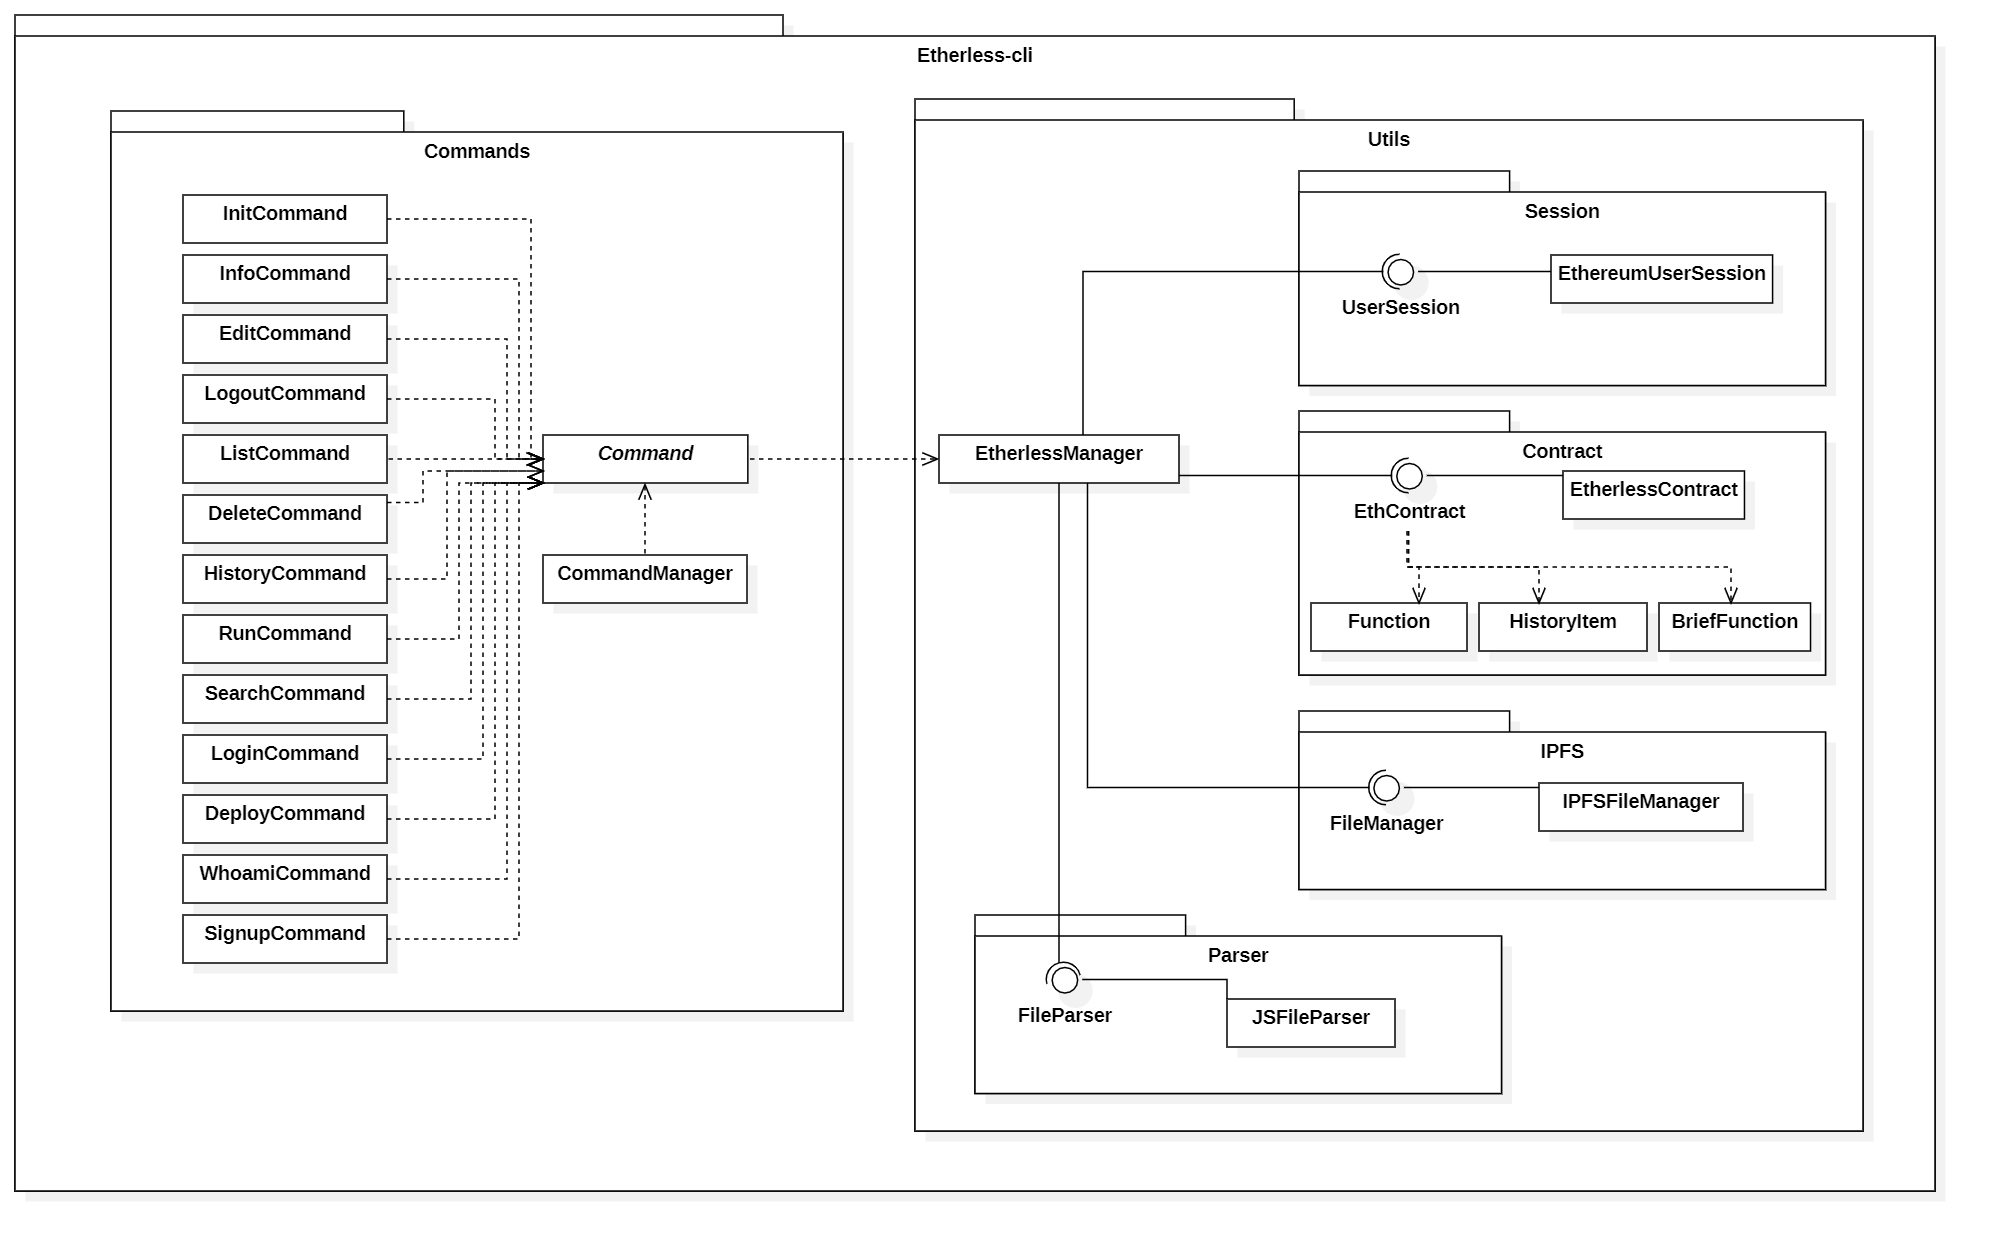
\includegraphics[scale=0.3]{diagrammi/etherless-cli/package.png}
\end{landscape}

\centerline{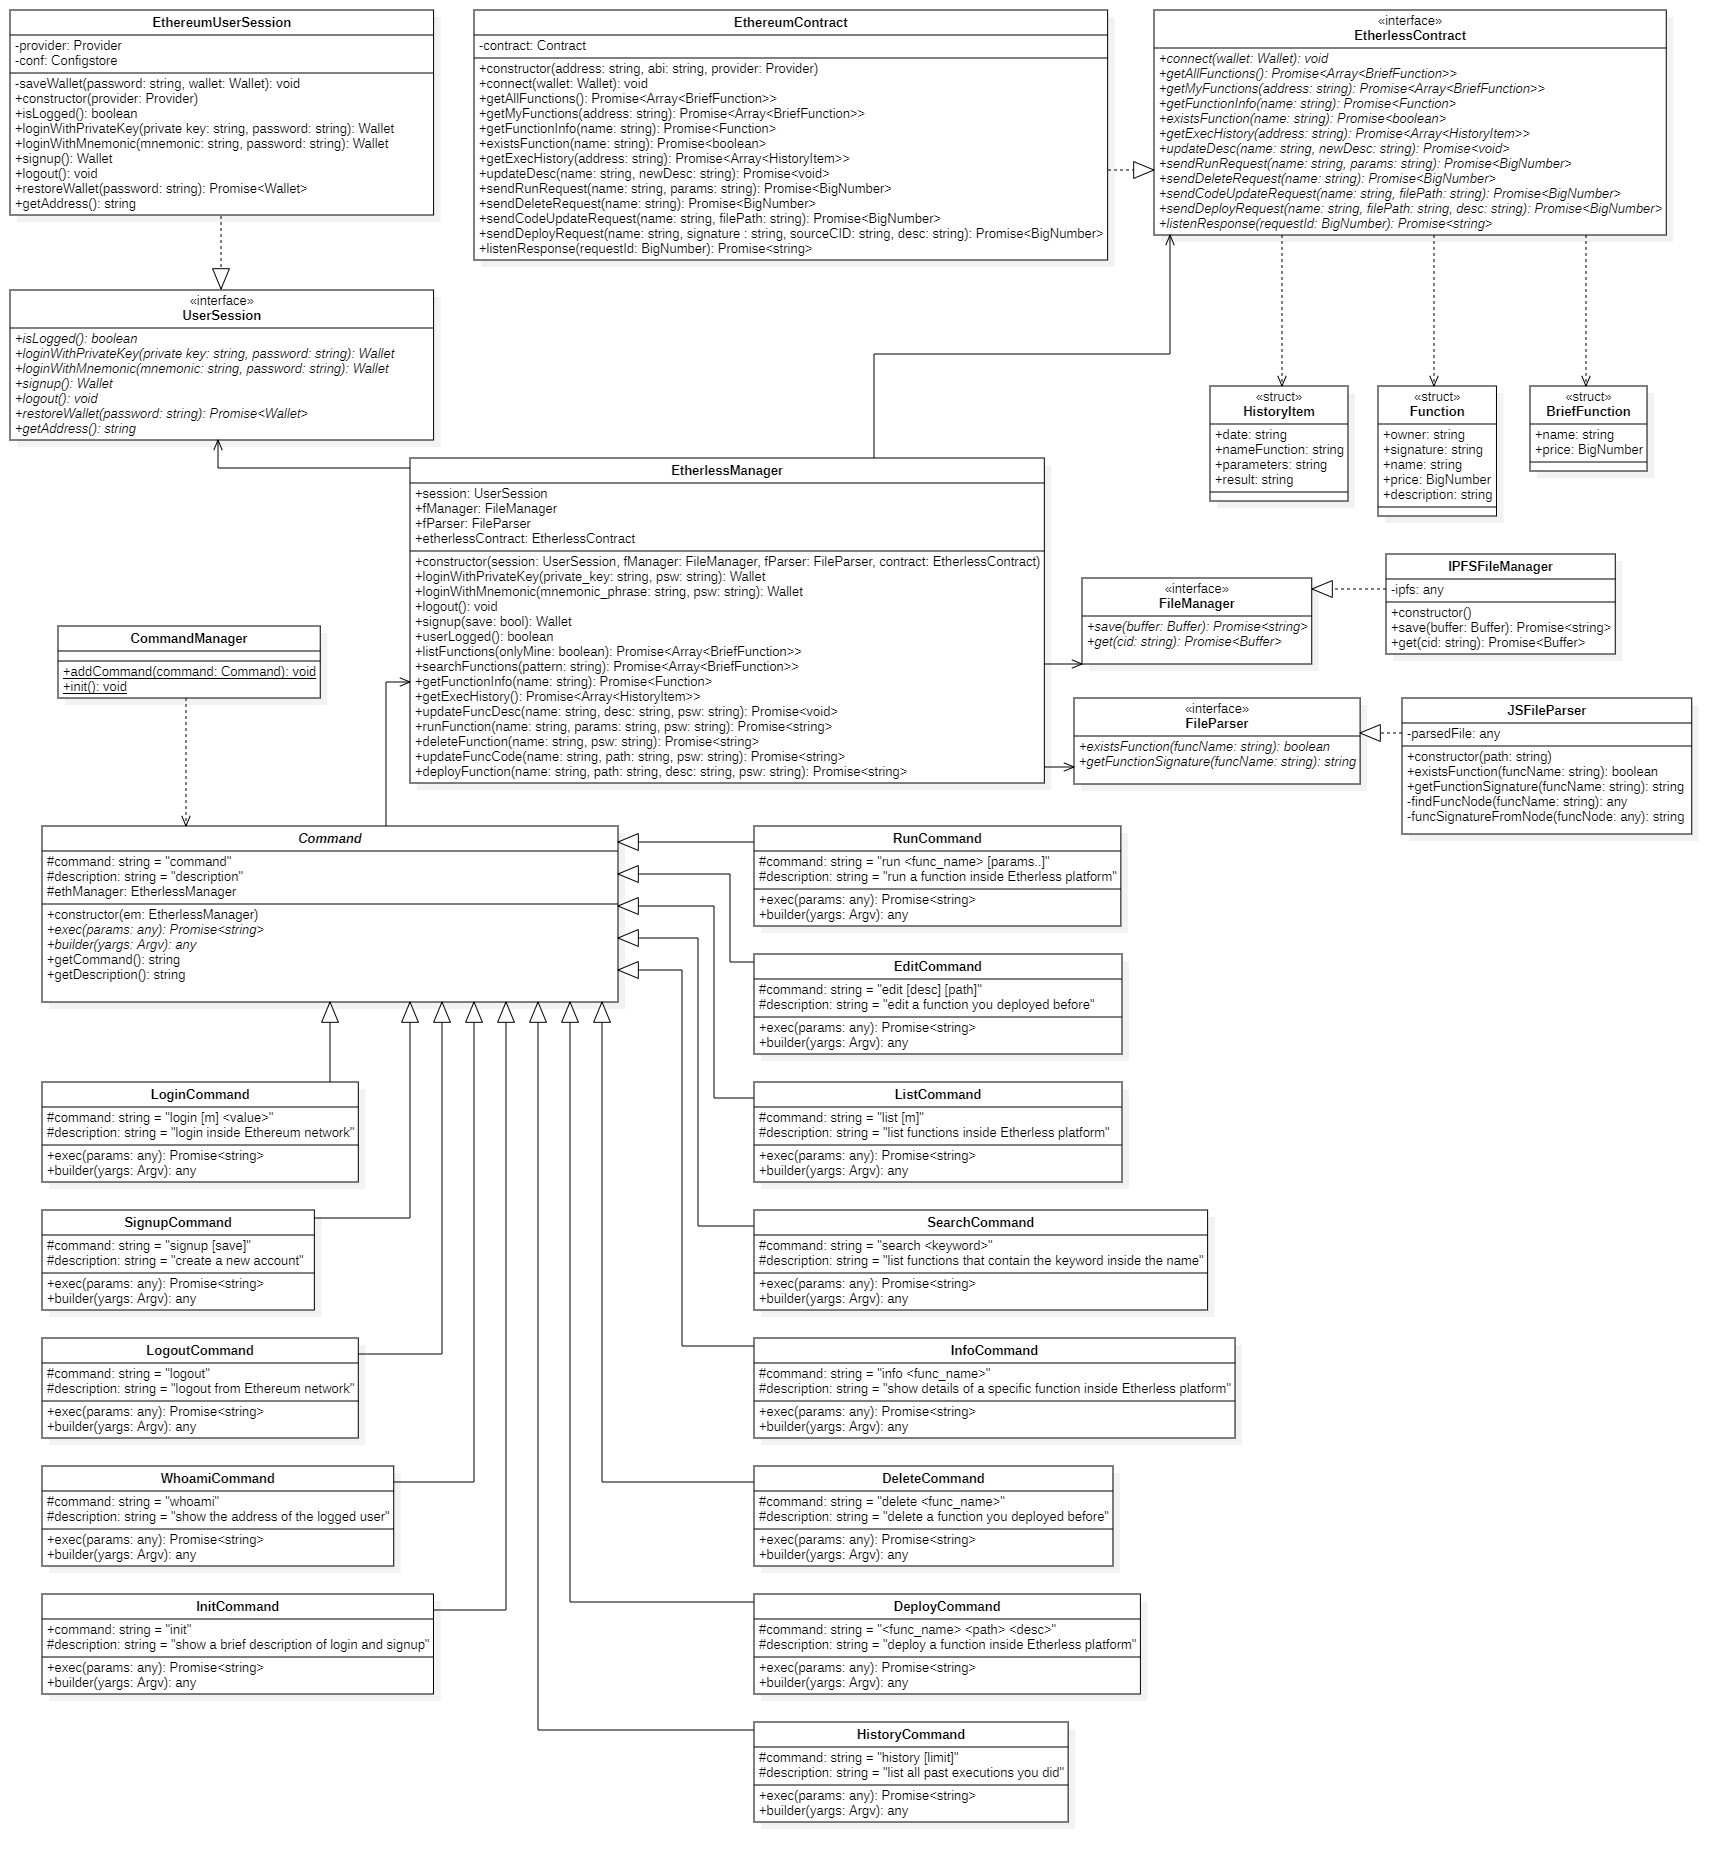
\includegraphics[height=19cm, width=16cm]{diagrammi/etherless-cli/classi.png}}

\subsubsection{Diagrammi di sequenza}
\begin{figure}[H]
	\noindent
	\makebox[\textwidth]{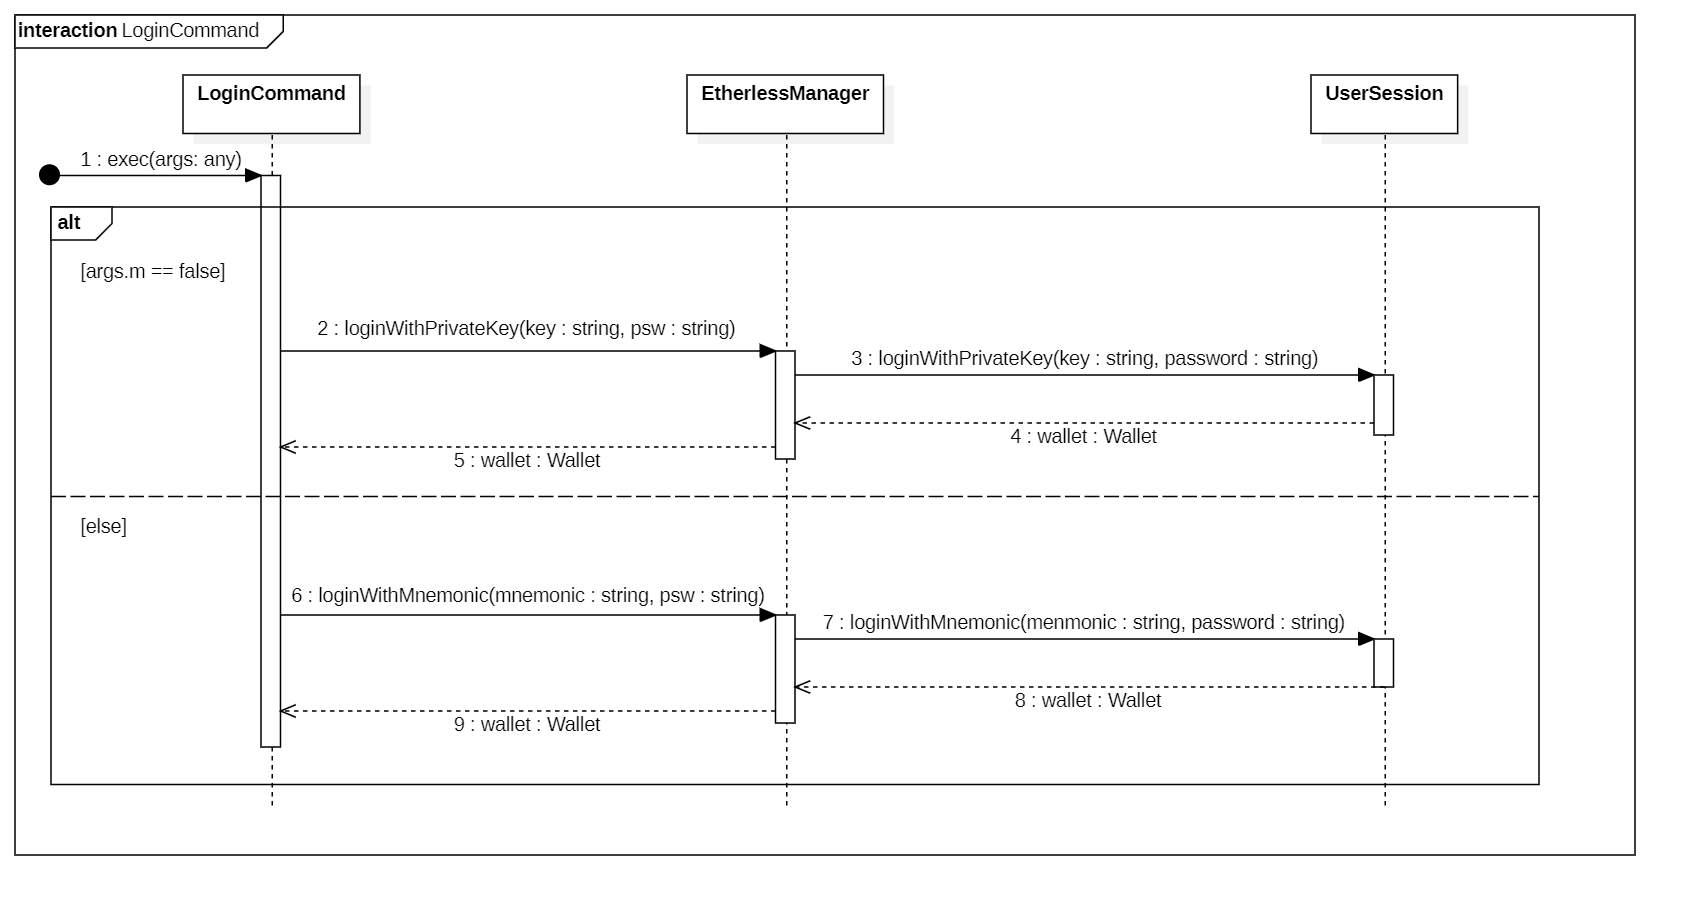
\includegraphics[scale=0.25]{././diagrammi/etherless-cli/loginCommand.png}}
	\caption{Diagramma di sequenza della procedura di autenticazione.}
\end{figure}
\begin{figure}[H]
	\noindent
	\makebox[\textwidth]{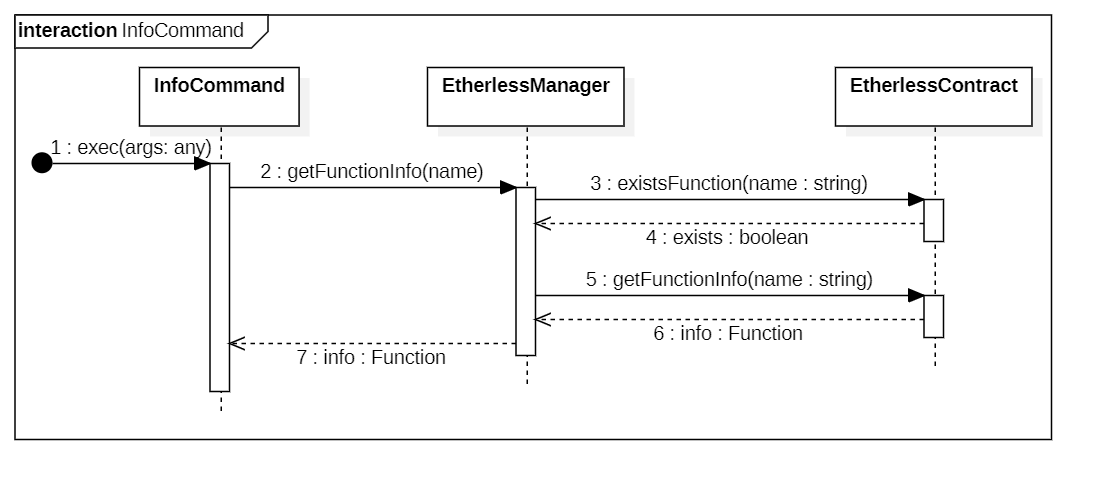
\includegraphics[scale=0.25]{././diagrammi/etherless-cli/infoCommand.png}}
	\caption{Diagramma di sequenza per le informazioni dettagliate di una funzione.}
\end{figure}
\begin{figure}[H]
	\noindent
	\makebox[\textwidth]{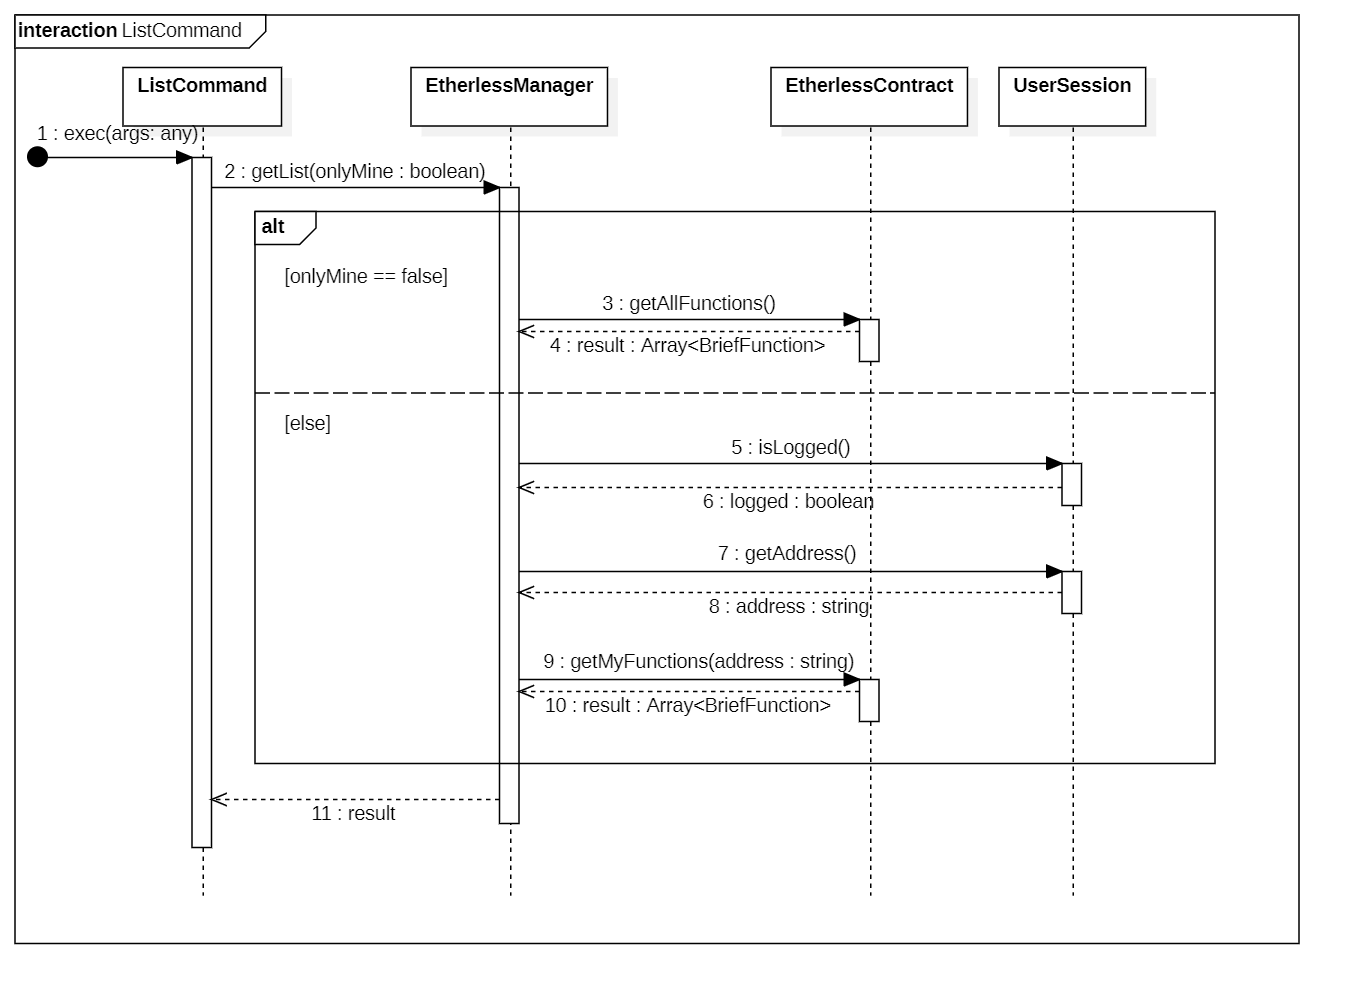
\includegraphics[scale=0.2]{././diagrammi/etherless-cli/listCommand.png}}
	\caption{Diagramma di sequenza per la lista delle funzioni disponibili.}
\end{figure}
\begin{figure}[H]
	\noindent
	\makebox[\textwidth]{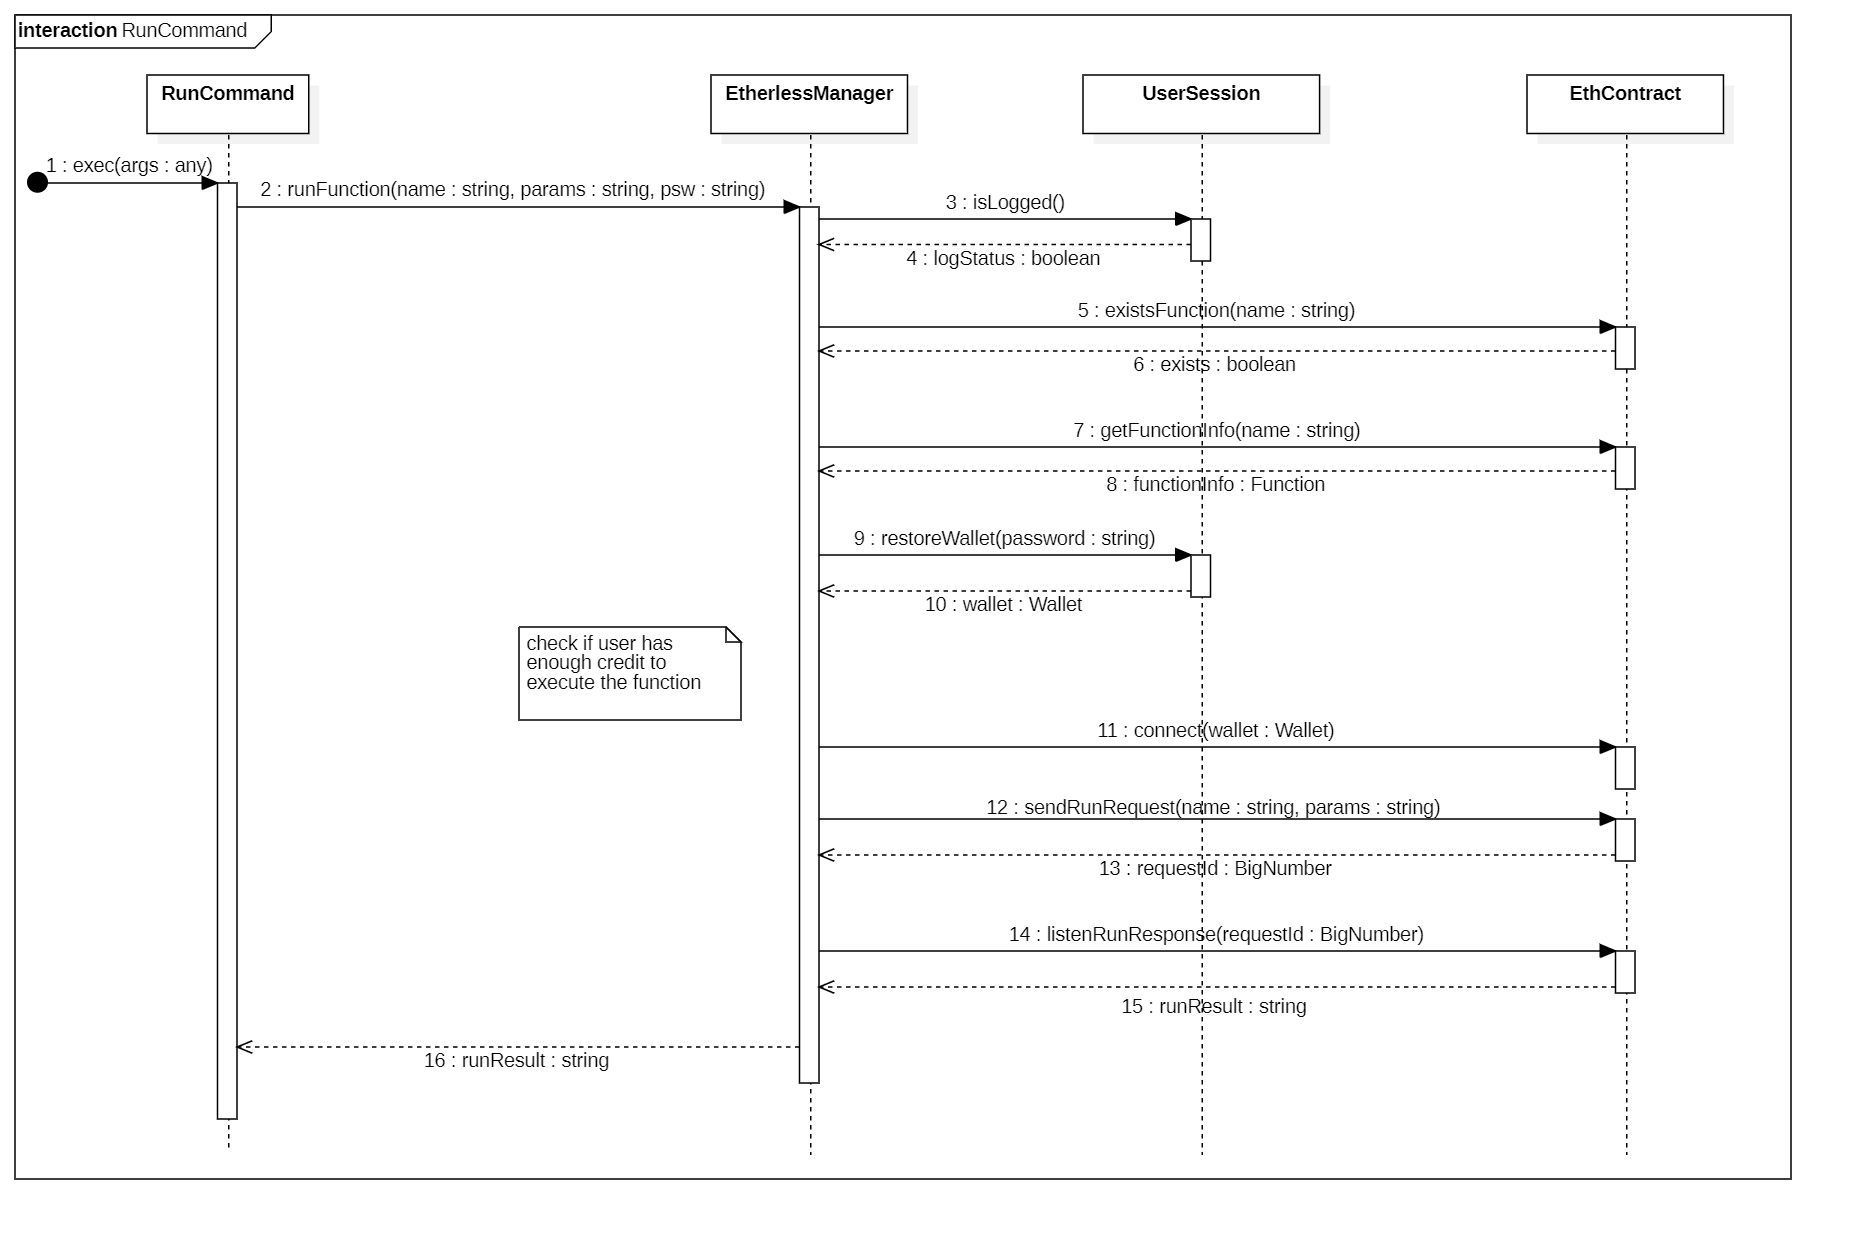
\includegraphics[scale=0.2]{././diagrammi/etherless-cli/runCommand.png}}
	\caption{Diagramma di sequenza dell'esecuzione di una funzione.}
\end{figure}
\begin{figure}[H]
	\noindent
	\makebox[\textwidth]{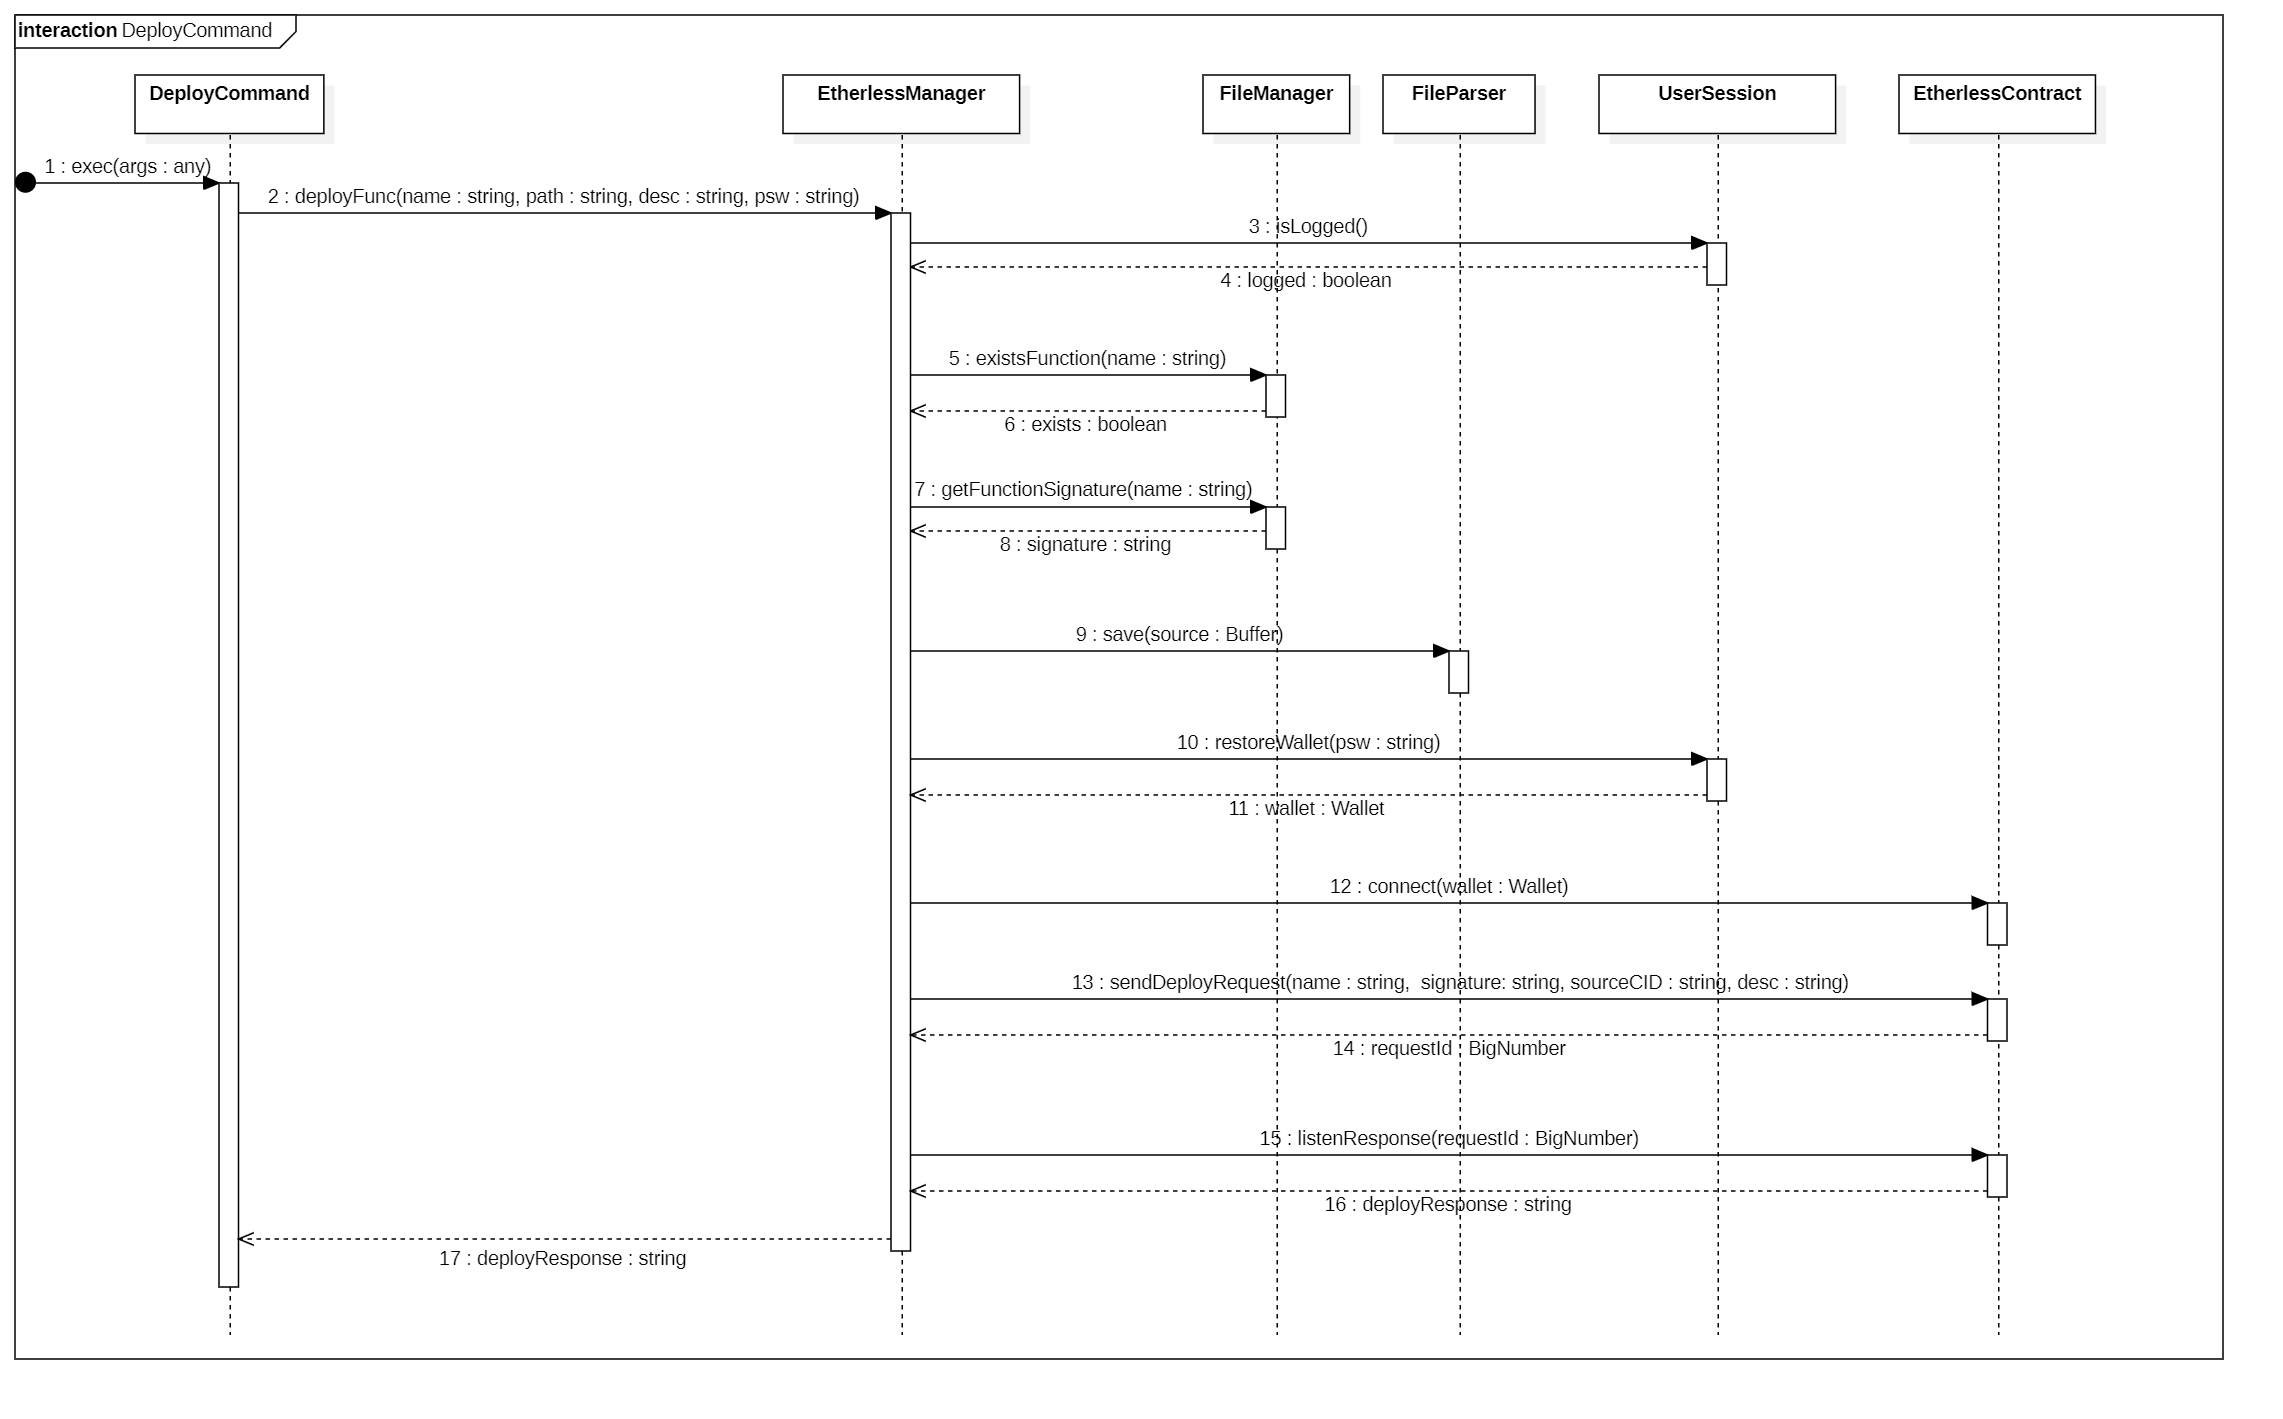
\includegraphics[scale=0.25]{././diagrammi/etherless-cli/deployCommand.png}}
	\caption{Diagramma di sequenza del deploy di una funzione.}
\end{figure}
\begin{figure}[H]
	\noindent
	\makebox[\textwidth]{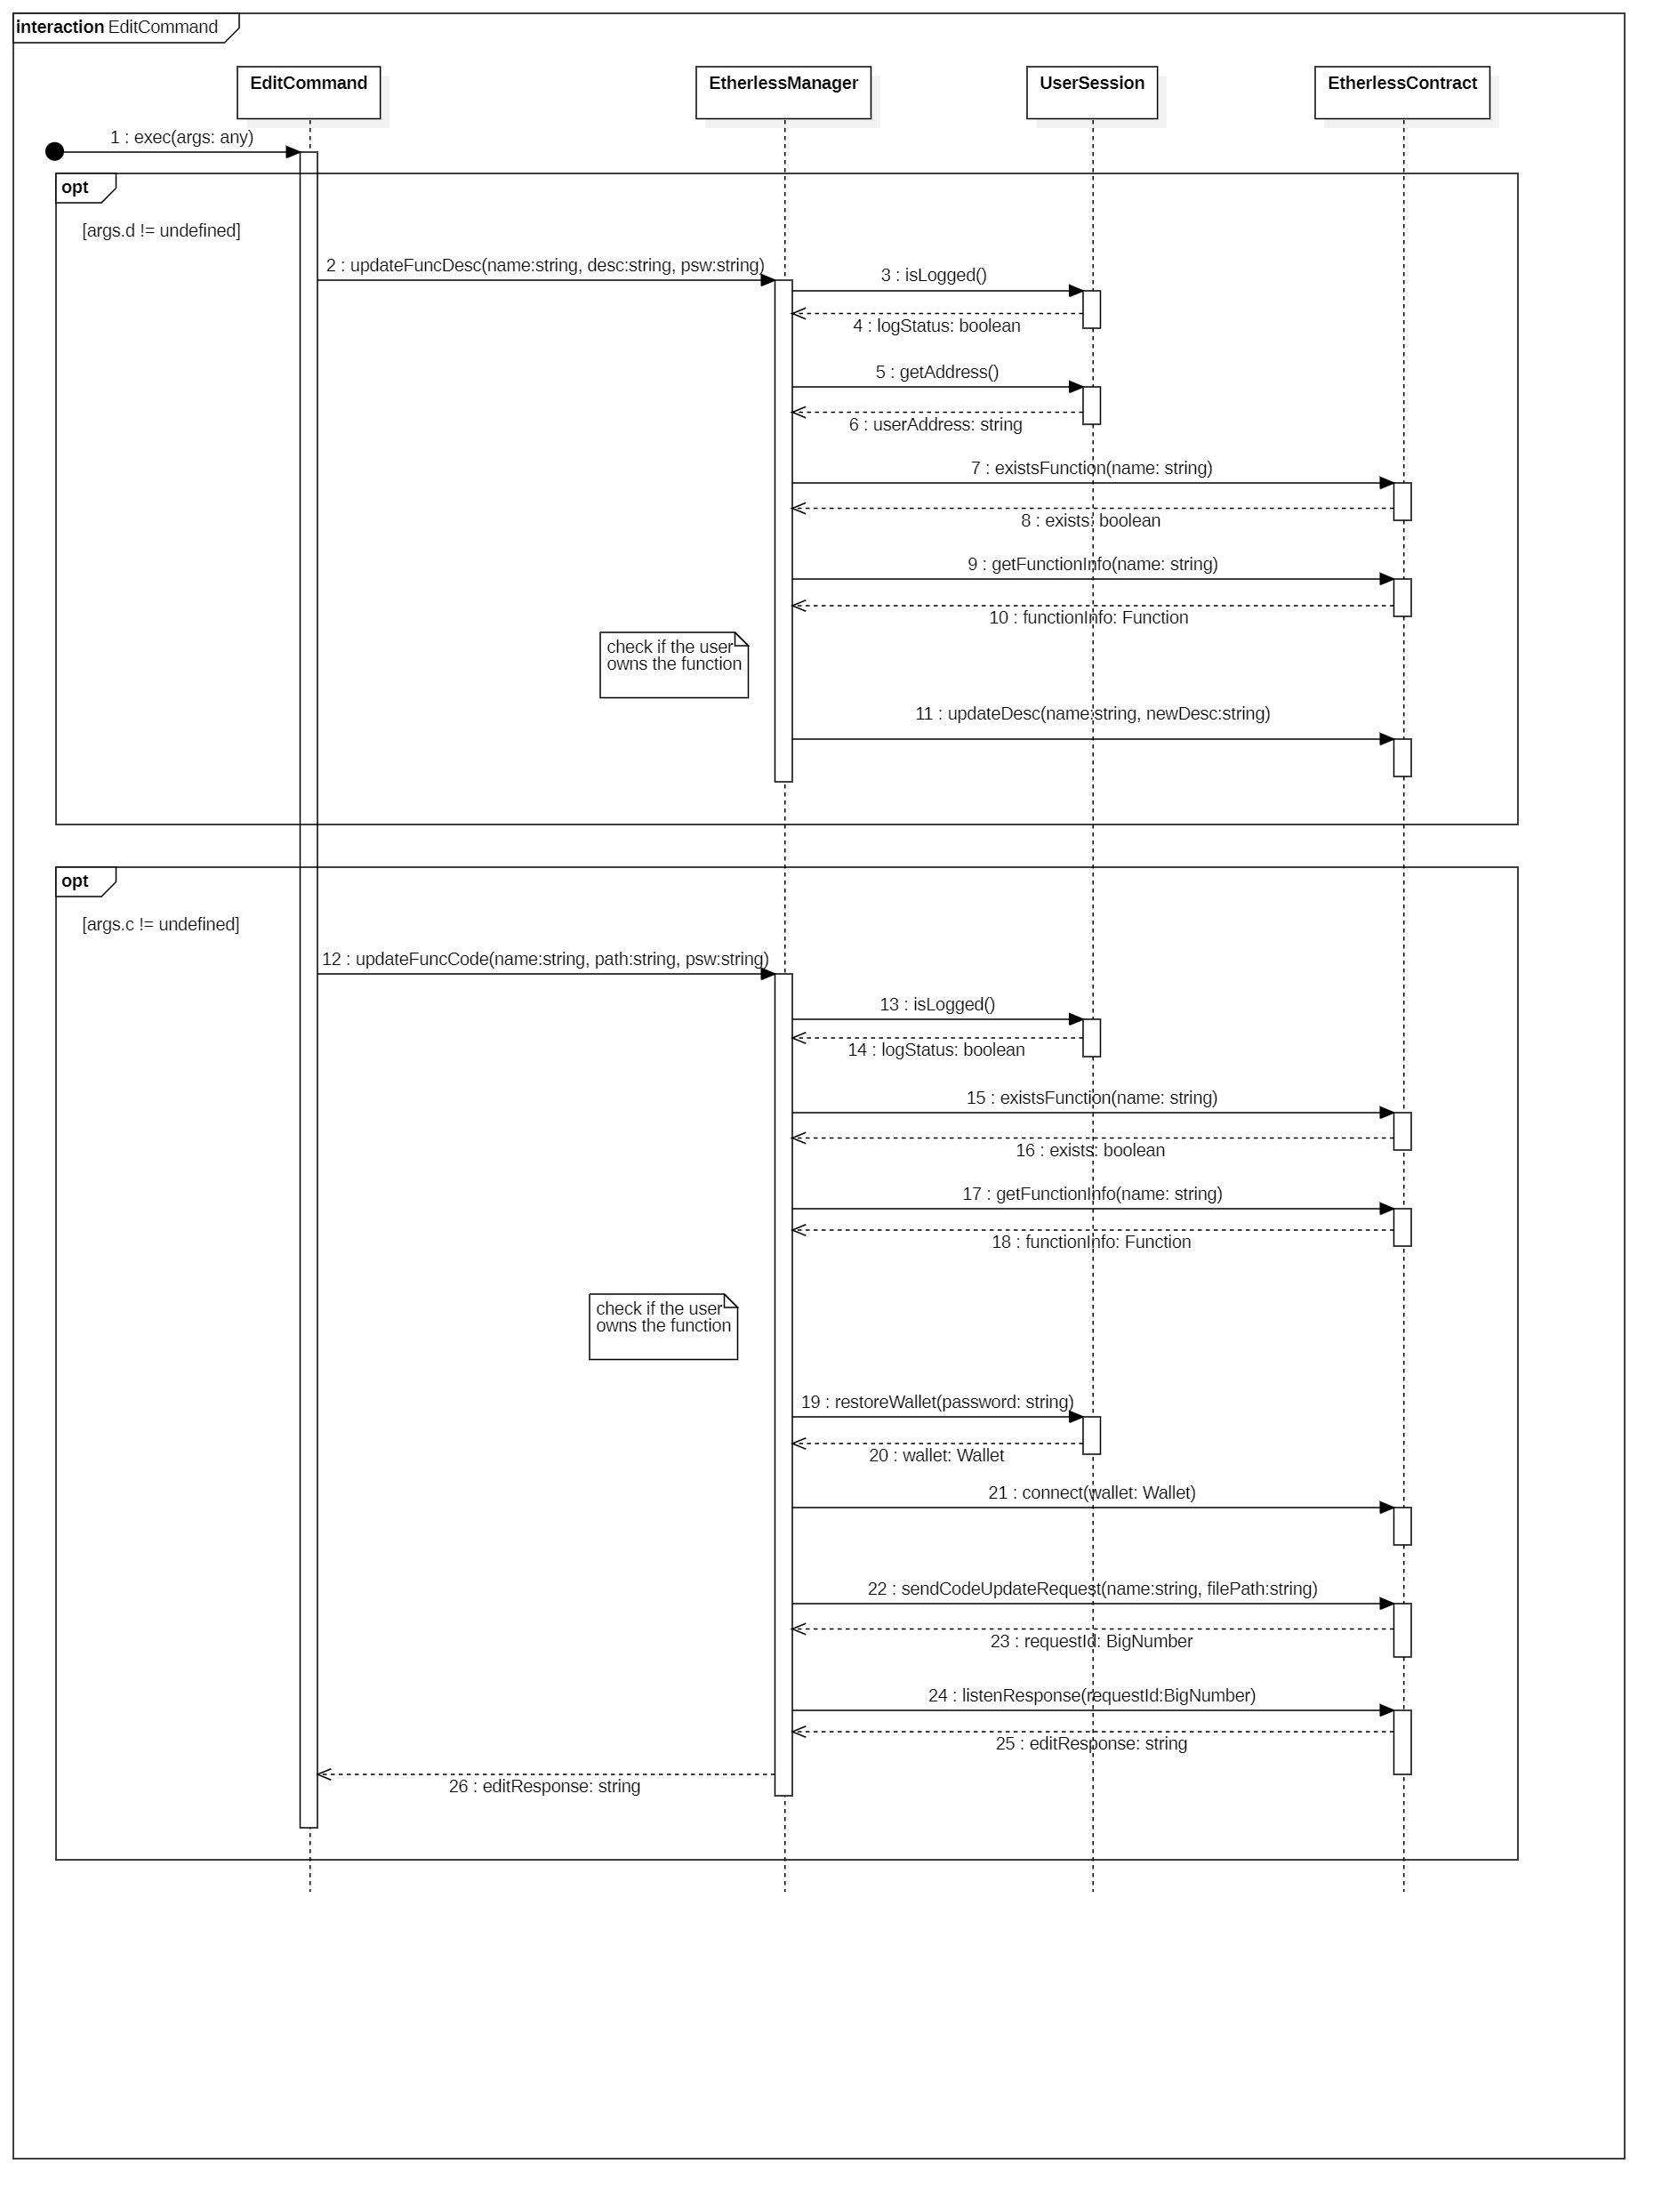
\includegraphics[scale=0.25]{././diagrammi/etherless-cli/editCommand.png}}
	\caption{Diagramma di sequenza della modifica di una funzione.}
\end{figure}

\begin{figure}[H]
	\noindent
	\makebox[\textwidth]{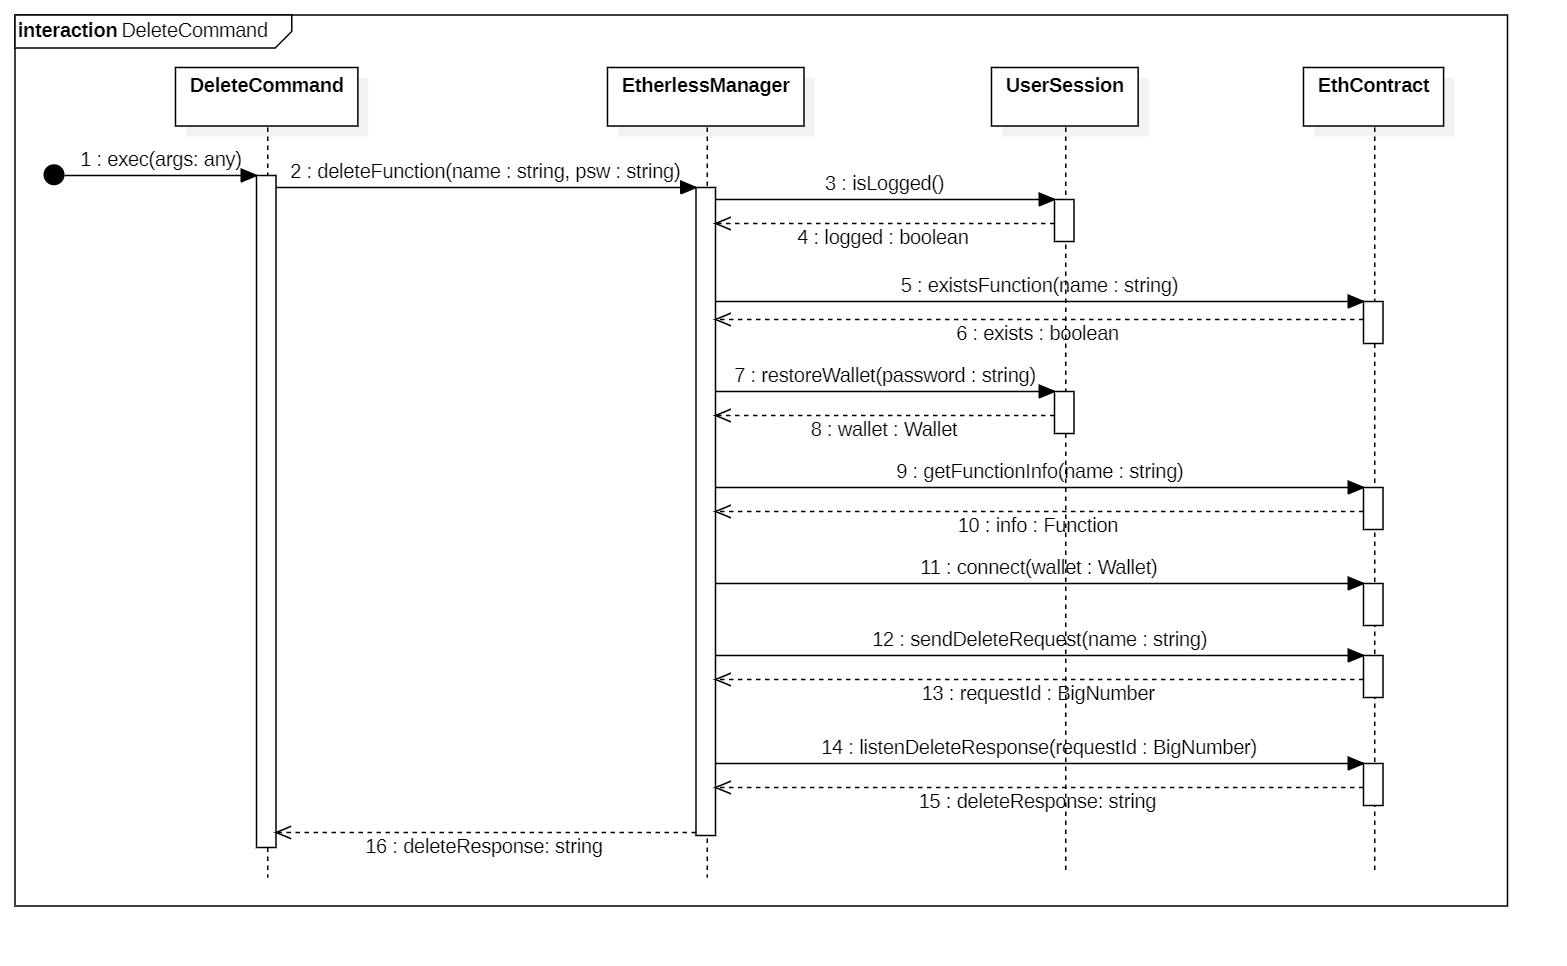
\includegraphics[scale=0.25]{././diagrammi/etherless-cli/deleteCommand.png}}
	\caption{Diagramma di sequenza dell'eliminazione di una funzione.}
\end{figure}


